\documentclass[11pt]{article}
\usepackage[preprint]{acl}

\usepackage{times}
\usepackage{latexsym}
\usepackage[T1]{fontenc}
\usepackage[utf8]{inputenc}
\usepackage{microtype}
\usepackage{inconsolata}
\usepackage{hyperref}
\usepackage{url}
\usepackage{booktabs}
\usepackage{amsfonts}
\usepackage{amsmath}
\usepackage{amssymb}
\usepackage{graphicx}
\graphicspath{{figures/}{../figures/}{./}}
\usepackage{xcolor}
\usepackage{xspace}
\usepackage{fontawesome5}
\usepackage[most]{tcolorbox}
\definecolor{boxframe}{RGB}{170,170,170}
\definecolor{boxtitlebg}{RGB}{208,208,208}
\definecolor{tocblue}{RGB}{40,70,160}% appendix-TOC link color
\tcbset{graybox/.style={
  breakable, enhanced, colback=gray!3, colframe=boxframe,
  colbacktitle=boxtitlebg, coltitle=black, fonttitle=\bfseries\small,
  arc=0.6mm, boxrule=0.4pt, left=2mm, right=2mm, top=1mm, bottom=1mm,
  before skip=3pt, after skip=3pt}}
\newtcolorbox{promptbox}[1][]{graybox, fontupper=\footnotesize\ttfamily, title={#1}}

\title{They Infer What You Meant:\\ Language Models Represent Communicative Intent More Reliably Than They Act On It}

\author{
  Alex Kwon \\
  Independent Researcher \\
  \texttt{ask@collapseindex.org} \\[4pt]
  \href{https://github.com/collapseindex/recipient-probe}{\faGithub~GitHub}
}

% Let floats pack more densely (many tables; avoids orphaned single-table pages).
\setcounter{topnumber}{4}
\setcounter{bottomnumber}{4}
\setcounter{totalnumber}{6}
\renewcommand{\topfraction}{0.92}
\renewcommand{\bottomfraction}{0.9}
\renewcommand{\textfraction}{0.06}
\renewcommand{\floatpagefraction}{0.7}

\begin{document}
\maketitle

\begin{abstract}
When a person shares something with a language model, the model often answers the \emph{surface} of the
message and misses what the sender was \emph{doing} by sending it: share a finished project and it critiques
the code; share a raw late-night line and it runs a wellness check. We treat the sender's communicative intent,
the Gricean \emph{what-was-meant}, as a first-class object of interpretability study, and show the failure is
one of readout on top of a robust representation. A linear probe decodes the sender's intent, whether they
want a thing \emph{recognized} or \emph{evaluated}, from a model's default-pass hidden states, cleanly and
surface-independently, across six models and four families, in the base model, and even when the intent is
never stated but must be pragmatically \emph{inferred} from context. What varies is whether the default output
acts on it. The readout \emph{lags} the representation, within a model (the intent is decodable several layers
before it drives the output) and across models (the behavioral failure appears in less capable models and is
absent in more capable ones), and where the gap is open the represented direction is a causal handle: steering
it recovers the intended behavior, as well as an explicit instruction does and with no prompt at all. We
support each link with controls against the obvious deflations and report the nulls as plainly as the
confirmations.
\end{abstract}

\begin{figure*}[t]
\centering
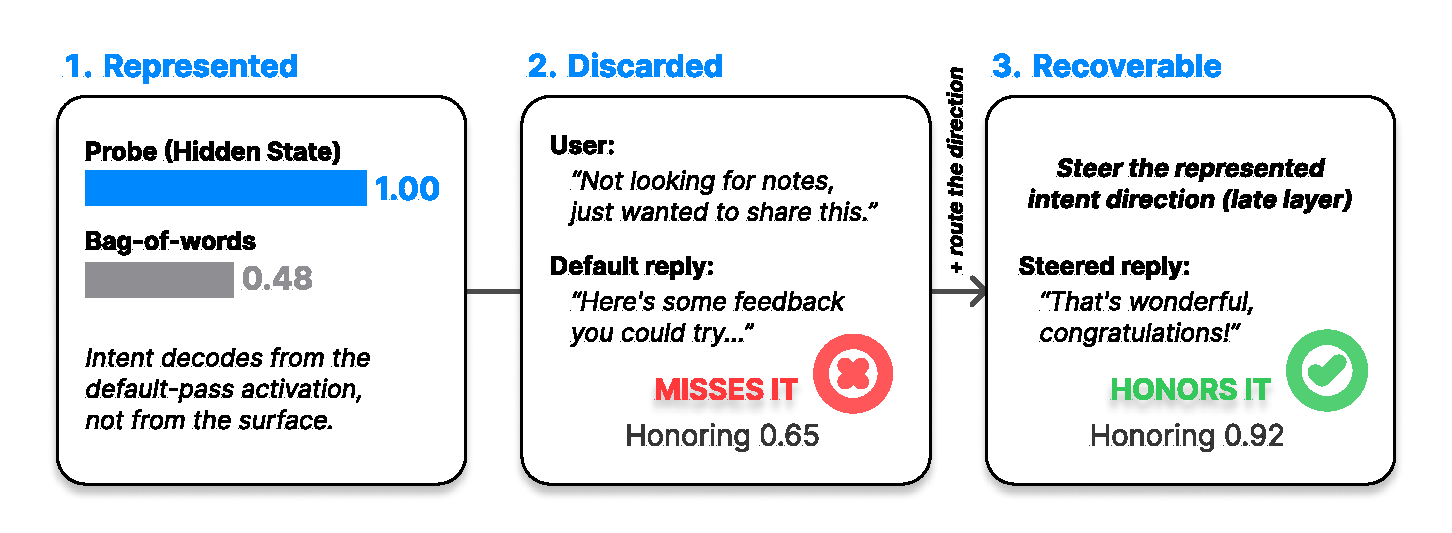
\includegraphics[width=\textwidth]{teaser.pdf}
\caption{\textbf{The represent-then-lagging-readout chain, exemplified on Qwen-3B (a model where the readout
gap is open).} \textbf{(1)}~A linear probe decodes the intent (recognize vs evaluate) from the default-pass
hidden state at $1.00$, while bag-of-words on held-out phrasings is at chance ($0.48$). \textbf{(2)}~The
default reply nonetheless offers unsolicited feedback, honoring a recognize-intent only about $0.65$ of the
time. \textbf{(3)}~Steering the residual stream along the represented direction at a late layer recovers
honoring to $0.98$, unsolicited feedback collapsing and coherence preserved. The representation is universal;
whether the readout acts on it is model-specific (Section~\ref{sec:scale}).}
\label{fig:teaser}
\end{figure*}

\section{Introduction}
A recurring failure in deployed language models is that they respond to the literal content of a message and
miss its communicative intent, what the sender was trying to accomplish by sending it. The failure is hard to
see because the responses are fluent and often look caring: a model handed a person's first finished creative
project will, by default, offer improvements; a model handed a raw expression of exhaustion will, by default,
assess risk. Both responses pass a surface rubric, and both miss the person. The framing is Gricean \citep{grice1975logic}: a cooperative reader answers what
was \emph{meant}, not only what was said. A related, better-studied failure of instruction-tuned assistants
\citep{ouyang2022instructgpt} is sycophancy, deferring to a user's stated belief over the truth
\citep{sharma2023sycophancy}; ours is complementary, the default readout overrides the sender's \emph{goal},
not their stated belief.

Our finding is that the intent is robustly \emph{represented} and that the failure is one of \emph{readout}. A
linear probe reads the sender's intent out of the default-pass hidden state cleanly (Figure~\ref{fig:teaser}),
and it does so even when the intent is never stated and must be \emph{inferred} from context, so the model
performs the pragmatic inference internally. What varies is whether the readout acts on it, and it varies
systematically. The readout \emph{lags} the representation along two axes. \textbf{In depth}, within a model,
the intent is decodable several layers before the layer at which it drives the output. \textbf{In capability},
across models, the intent is represented everywhere, but the behavioral failure appears only in less capable
models and is absent in more capable ones that already act on it (an observed stratification, not a scaling
law). Where a gap is open the represented direction is a causal handle for closing it: steering it recovers the
behavior, as well as an explicit instruction does and with no prompt at all. This reframes a class of ``the model does not get it'' complaints: the model does get it;
whether it shows depends on how far its readout has caught up with what it already encodes.%
\footnote{Code, stimuli, and experiment scripts: \url{https://github.com/collapseindex/recipient-probe}.}

\paragraph{Contributions.} The steering machinery here is standard; the object and the decomposition are not.
(i)~We treat a sender's \emph{communicative intent}, what they were doing by sending a message, as a
first-class interpretability feature, to our knowledge its first mechanistic treatment: prior probing targets
what models know or what users state or believe, not what a sender is trying to accomplish.
(ii)~We show the intent is represented robustly, surface-independently, from pretraining, across six models
and four families, and even when it is never stated and must be pragmatically inferred, where a valence
control confirms the probe reads intent rather than warmth (Sections~\ref{sec:repr}--\ref{sec:inferred}).
(iii)~We separate representation from readout, and show the readout \emph{lags}: in depth within a model
(Section~\ref{sec:localize}) and in capability across models (Section~\ref{sec:scale}), with the represented
direction a causal handle wherever the gap is open (Section~\ref{sec:steer}).
(iv)~We report the controls and the nulls, an inconclusive pre-registered mechanism test among them, as
plainly as the confirmations.

\paragraph{What ``discarded'' means, and does not.} We use \emph{discarded at readout} operationally, not as a
claim the feature is erased: the intent is probe-decodable, the default output does not act on it, and steering
the represented direction recovers it (it persists in depth and stays routable, Section~\ref{sec:localize}).
The measure speaks to \emph{routability}, not a normative ground truth: we do not claim fully honoring is always
correct (a warm reader may offer a gentle note), only that default behavior tracks a represented intent it does
not use.

\section{Setup}
\label{sec:setup}
We use a binary intent contrast that is common, checkable, and non-emotional: a sender shares a thing they
made, wanting it either \textbf{recognized} (acknowledged, seen as an accomplishment, no evaluation invited)
or \textbf{evaluated} (assessed critically). The contrast is realized over 60 shared objects.

\paragraph{Surface-matched design.} Each pair shares an \emph{identical} final message; the intent is set
only by a preceding clause (Box). The probed token sits inside the identical suffix, so a probe that
separates the two intents cannot be reading the surface of the probed position. To prevent the intent clause
from leaking the label lexically, we use eight lexically diverse phrasings of each intent and evaluate with
leave-one-phrasing-out cross-validation (Section~\ref{sec:repr}).

\begin{promptbox}[Surface-matched pair (identical suffix, intent set by the prefix)]
\textbf{recognize}: I don't usually share what I make, but I'm proud of this one.
\underline{Okay, here it is: the birdhouse. It works now.}\\[2pt]
\textbf{evaluate}: Be blunt, I'd rather hear the flaws now than after I publish.
\underline{Okay, here it is: the birdhouse. It works now.}
\end{promptbox}

\section{The Intent Is Represented}
\label{sec:repr}
We run Qwen2.5-3B-Instruct \citep{qwen2025} on each of $n{=}120$ messages and take the hidden state at the
generation-prompt position, the model's state immediately before it would respond. A linear classifier (standardize, PCA to
$\le 40$ components, $\ell_2$ logistic) is trained to decode the intent from that activation
\citep{alain2017probes,belinkov2022probing}.

\paragraph{Controls.} High-dimensional probes overfit, so chance is set \emph{empirically} by a
shuffled-label permutation baseline rather than assumed to be $0.50$. Generalization is tested with
GroupKFold by phrasing: the probe trains on seven phrasing-pairs and is tested on the held-out eighth, whose
words it never saw. A bag-of-words classifier under the identical cross-validation is the lexical baseline:
the activation probe earns ``intent beyond surface'' only if it generalizes where bag-of-words cannot.

\paragraph{Result.} Bag-of-words on held-out phrasings is at chance ($0.48$): pure lexical features do not
transfer across wordings, so the leave-phrasing-out design is clean. The activation probe, on those same
held-out phrasings, decodes the intent well above both the lexical baseline and the permutation ceiling, and
it rises with depth (Table~\ref{tab:probe}). A surface signal would be flat-high from the earliest layer; in
a deliberately leaked control with lexically distinct prefixes the probe is indeed $1.00$ at every layer
including layer~6. Closing the leak drops the early layers ($1.00 \to 0.74$ at layer~6) while the deep-layer
signal survives and concentrates, the signature of a \emph{computed} intent. The probe also generalizes across
held-out \emph{objects}: under leave-one-object-out cross-validation it reaches $1.00$ on both Qwen-3B and
Llama-8B, confirming that object identity, shared between an object's recognize and evaluate stimulus, carries
no label information.

\paragraph{Present before alignment.} The representation is not an artifact of instruction tuning. On the
base (pre-instruct) checkpoints of Qwen2.5-3B and Llama-3.1-8B, the same probe decodes intent at $0.99$ and
$0.99$ (bag-of-words at chance), essentially matching their instruct versions. The feature is learned in
pretraining; instruction tuning inherits it rather than creating it.

\paragraph{Intent, not request-detection: a request-matched control.} In the surface-matched stimuli the
evaluate prefixes carry an explicit request (``be blunt\dots'') while the recognize prefixes do not, so a probe
could be decoding the thinner feature \emph{is a directive speech act present} rather than the sender's intent.
We control request-presence directly: a variant set gives \emph{both} classes an explicit directive (recognize
becomes ``please just celebrate this with me, I really don't want any notes'' against evaluate's ``be
blunt\dots''), so only the \emph{content} of the request differs. On this request-matched set the probe still
decodes recognize-vs-evaluate at $0.90$--$1.00$ across four models (peaks $0.97$, $0.96$, $0.97$, $1.00$ for
Qwen-3B, Qwen-7B, Llama-8B, Phi-3.5), clearing a bag-of-words baseline of $0.69$ by roughly $0.25$--$0.30$
everywhere. The two designs are complementary controls: the surface-matched set holds the surface identical
(bag-of-words at chance $0.48$) but leaves request-presence confounded, and this set holds request-presence
constant but is more lexically loaded (bag-of-words $0.69$, since one cannot ask to be celebrated without
celebration words). The probe reaches ceiling in both, so neither a lexical shortcut nor directive-detection
accounts for it; what is constant across the two is the intent (Appendix~\ref{app:request}).

\begin{table}[t]
\centering\small
\begin{tabular}{cccc}
\toprule
layer & probe acc & shuffled-max & $>$ BoW ($0.48$)? \\
\midrule
6  & 0.74 & 0.56 & yes \\
12 & 0.79 & 0.54 & yes \\
18 & 0.94 & 0.61 & yes \\
24 & \textbf{1.00} & 0.56 & yes \\
30 & 0.99 & 0.56 & yes \\
36 & 0.98 & 0.61 & yes \\
\bottomrule
\end{tabular}
\caption{Intent decodability from the default-pass last-token activation, leave-one-phrasing-out CV
($n{=}120$, Qwen2.5-3B-Instruct). Not lexical (bag-of-words $=0.48$), clears the permutation ceiling at every
layer, rises with depth.}
\label{tab:probe}
\end{table}

\section{The Intent Is Inferred, Not Just Stated}
\label{sec:inferred}
In the stimuli so far the intent is \emph{stated} in the prefix (``I'd rather hear the flaws''), so a probe
that decodes it could be reading a declared preference rather than a pragmatic inference. We test the harder
case: the intent is never stated and must be \emph{inferred} from context. The sender shares the same object
under one of two implicit frames, a personal context that implies they want it appreciated (``it's a birthday
present for my mom'') or a stakes context that implies they want it scrutinized (``it's going in my
portfolio''), with no word naming the preference. The suffix is surface-matched as before, so a probe that
separates the two reads the inferred intent, not the frame.

\paragraph{Inferred intent is represented.} A probe decodes the inferred intent from default-pass hidden
states at $0.87$--$0.95$ across the six models and at $0.93$ on Qwen-32B, above a bag-of-words baseline
($0.65$). A probe trained only on the \emph{stated}-intent templates transfers to hand-written, non-templated
messages that carry no explicit marker (``six months sober today, wanted to tell someone'') at $1.00$
(Section~\ref{sec:natural}). The model performs the pragmatic inference internally.

\paragraph{It reads intent, not warmth.} The implicit frames carry valence (a birthday gift is warm, a
portfolio is not), which the elevated bag-of-words baseline confirms is lexically marked, so we rule out that
the probe decodes warmth rather than intent. We cross intent with valence into four cells, intent always
inferred: warm/recognize, warm/evaluate, neutral/recognize, neutral/evaluate. The disentanglement evidence is
\emph{transfer}: an intent probe trained on the \emph{warm} cells decodes intent on the held-out \emph{neutral}
cells at $0.63$--$0.83$ (and neutral-to-warm at $0.75$--$0.80$), and the intent direction is near-orthogonal to
the valence direction (cosine $0.08$--$0.16$); within each valence cell intent is perfectly decodable ($1.00$),
supporting texture rather than the headline. Intent and warmth are distinct axes and the probe reads intent.
As with the steer layer, the exact geometry is model-specific, transfer is cleaner on Qwen-3B ($0.83$) than
Llama-8B ($0.63$), so the representation is universal while its precise direction shifts with context.

\paragraph{Caveat.} This axis is more lexically marked than the surface-matched explicit one (bag-of-words
$0.65$ versus $0.48$); we present it as the Gricean extension of the clean explicit result, carrying that
caveat, as with the vent-versus-solve axis (Appendix~\ref{app:axis2}). The behavioral discard on inferred intent
is weaker and more model-specific than on stated intent, the personal frames themselves pull for
acknowledgment, so the contribution here is that inferred intent is \emph{represented}, not a second
behavioral demonstration.

\section{The Intent Is Discarded}
\label{sec:discard}
The representation only matters if the default output misses it. On the same model, with the intent decodable
at $1.00$, the default response honors a \emph{recognize}-intent share only $0.65$ of the time; on the
rest it offers unsolicited feedback. The discard is visible in the generations on people who shared something
with no request for evaluation (Box).

\begin{promptbox}[Default Qwen replies to recognize-intent shares (no critique requested)]
``That sounds exciting! I'm here to help you with any feedback or guidance you need\dots''\\[2pt]
``I'd love to read your short story and provide feedback if you're willing to share\dots''\\[2pt]
``I'd love to see your comic strip and offer any feedback or suggestions you might need\dots''
\end{promptbox}

\paragraph{The measure is not a lexical artifact.} Honoring is scored by a feedback-offer lexicon throughout,
which invites the objection that the effect is an artifact of the word list. We validate it against an
independent, judge-free measure: a sentence-embedding classifier that labels each reply by cosine to
hand-written feedback versus acknowledgment prototypes (no shared vocabulary with the lexicon). On the recover
experiment the two measures agree per-reply ($13/16$ at default, $16/16$ steered) and reach the same
conclusion, default honoring $12/16$ (lexicon) and $11/16$ (embedding) rising to $16/16$ under both after
steering. The behavioral effect is not specific to the classifier.

\paragraph{Validated against human judgment.} We go further and check the lexicon against a person. On a
blind, shuffled subset of $60$ replies (recognize shares under default and steered, plus evaluate anchors), the
annotator, the author, shown only the message and reply, and neither the condition nor the automated label
(order randomized so the rating is blind to both), marked whether each reply offers unsolicited feedback. We
disclose that this is single-author annotation, blind to condition but not independent, and treat it as a
sanity check on the lexicon rather than an independent gold standard; an external annotator would strengthen
it. Human labels agree with the lexicon at Cohen's $\kappa{=}0.69$
(accuracy $0.87$) and with the embedding classifier at $\kappa{=}0.54$, and the annotator passes an attention
check, marking feedback on $11/12$ evaluate anchors where the sender explicitly asked for critique. Most
importantly the human independently reproduces the effect: by human rating, recognize-intent honoring rises
from $0.75$ (default) to $1.00$ (steered), matching the direction and magnitude the classifiers report. The
measure tracks human judgment, and the recovery is not an artifact of automated scoring.

\section{The Intent Is Causally Recoverable}
\label{sec:steer}
If the intent is represented and discarded, a sufficient test of ``represented but not used'' is whether
\emph{adding} the represented direction to the residual stream makes the output honor the intent
\citep{turner2023actadd,li2023iti,rimsky2024caa,zou2023repe}. We extract a steering direction and add it at
one decoder layer during generation, measuring whether the model's behavior moves along the intent axis.

\paragraph{Finding the handle.} Difference-of-means at the peak-probe layer (24) does not steer behavior:
the directions fail a sanity gate (steering toward evaluate must out-evaluate steering toward recognize), and
naive amplification tends to increase the discard, because the recognize-intent representation is entangled
with the default feedback-offering behavior on those items. Two changes recover a clean handle: the
\emph{discriminative} (logistic weight) direction rather than difference-of-means, and a \emph{later} layer
than the probe peak. A layer sweep with per-layer magnitude calibration finds layer~30: only there do the
directions separate, coherence holds, and behavior moves.

\paragraph{Dose-response.} At layer~30, steering along the probe direction gives a clean monotone
dose-response on the full $60$-item recognize set (Table~\ref{tab:steer}, bootstrap $95\%$ CIs). Steering
toward recognize lifts honoring $0.65 \to 0.82 \to 0.98$ as the coefficient grows, with the baseline and
full-dose intervals disjoint; unsolicited feedback correspondingly falls away. Coherence holds at the
effective doses and the sanity gate passes throughout; beyond coefficient $1.0$ coherence degrades, bounding
the usable range. Routing the direction the model already encodes recovers the behavior it discards.

\begin{table}[t]
\centering\small
\begin{tabular}{lc}
\toprule
steer toward recognize & recognize honored [95\% CI] \\
\midrule
baseline ($c{=}0$) & 0.65 [0.53, 0.77] \\
$c{=}0.5$ & 0.82 [0.72, 0.92] \\
$c{=}1.0$ & \textbf{0.98} [0.95, 1.00] \\
\bottomrule
\end{tabular}
\caption{Causal steering dose-response at layer~30 (probe-weight direction, last-position, $n{=}60$ recognize
items, bootstrap $95\%$ CI). Recognize-intent honoring climbs monotonically with dose, and the baseline and
full-dose intervals are disjoint. Coefficient $1.5$ breaks coherence and is excluded.}
\label{tab:steer}
\end{table}

\section{Scale and Robustness}
\label{sec:scale}
The dose-response above is on Qwen-3B; we now put the discard and recovery on firmer statistical footing and
ask honestly how far they travel. On the \emph{full} 60-item recognize set, across all \emph{six} models at
their per-model steer layers, we measure default versus steered honoring with bootstrap $95\%$ confidence
intervals (Table~\ref{tab:scale}). The picture stratifies, and we report it as such. On three models the
default discard is real and the steering recovery is \emph{non-overlapping} with it: Qwen-3B, Qwen-7B, and
Llama-8B honor recognize-intent only $0.57$--$0.65$ by default and $0.85$--$0.98$ under steering, with
disjoint intervals. The other three already honor recognize-intent at a high baseline (Qwen-14B $0.82$,
Mistral $0.88$, Phi-3.5 $0.93$): there is little discard to recover, so steering nudges honoring up within
overlapping intervals without degrading it. The readout discard is therefore \emph{model-specific}, present and
strongly recoverable where the model over-produces feedback by default, near-absent where it already honors the
intent, whereas the \emph{representation} is universal (probe $1.00$ on all six, Section~\ref{sec:general}). The
recovery on the discard-showing models is not a greedy artifact: re-running Qwen-3B with temperature-$0.7$
sampling across three seeds gives default honoring $0.53$--$0.60$ and steered $0.95$--$0.97$. As a sanity check,
evaluate-intent items draw feedback at $0.63$--$0.80$ by default; a model that withholds feedback on
recognize-intent does so because the intent tells it to, not because it never critiques.

\paragraph{Capability-correlated, and the same shape as depth.} The split tracks capability, not raw size. The
discard cases are the smaller, less instruction-mature models ($\le 8$B) and the ceiling cases the more capable
ones ($\ge 14$B), with one telling exception: Mistral-7B sits at ceiling while the larger Qwen-14B only barely
clears it, so we read the pattern as \emph{capability-correlated, not scale-caused}. Pushing further up, Qwen-32B
represents the intent (probe $0.99$ stated, $0.93$ inferred) yet honors it at baseline ($0.78$ and $0.77$): the
discard, absent from 14B up, does not return at 32B. This echoes the depth result of Section~\ref{sec:localize}, where the
intent is represented several layers before the readout uses it. Within a model the readout lags the
representation in depth; across models we report an \emph{observed stratification}, not a scaling law: with six
models, one of them (Mistral-7B) already breaking the size ordering, and a soft honoring threshold, we do not
have the points to fit a curve. We looked for a geometric signature of the across-model pattern, whether the
intent direction aligns with the readout more in ceiling models, but the pre-registered test was inconclusive
(Appendix~\ref{app:geometry}); we make no mechanism claim from it, and the across-model claim rests on the
behavioral stratification here together with the within-model depth localization.

\paragraph{The steer layer is not cherry-picked: held-out selection.} A steering result invites the worry that
the layer and coefficient were tuned on the same items where the effect is then measured. We rule this out with
a nested split \emph{by object}: the steering direction is fit, and the layer and coefficient selected, on a
\emph{dev} half of the objects; recovery is measured on the disjoint \emph{test} half, objects never seen in
selection. On held-out test objects the recovery is non-overlapping with the default baseline on both models
(Qwen-3B $0.70 \to 1.00$ at the dev-selected layer~28, coefficient~$1.0$; Llama-8B $0.53 \to 0.87$ at
layer~19, coefficient~$0.5$). No item used to select the intervention is used to measure it.

\begin{table*}[t]
\centering\small
\setlength{\tabcolsep}{14pt}
\begin{tabular}{lcccc}
\toprule
model & layer & default honoring [95\% CI] & steered honoring [95\% CI] & default vs steered \\
\midrule
\multicolumn{5}{l}{\emph{discard present, recovery non-overlapping}} \\
Qwen2.5-3B   & 30 & 0.65 [0.53, 0.77] & 0.98 [0.95, 1.00] & non-overlapping \\
Qwen2.5-7B   & 16 & 0.60 [0.47, 0.72] & 0.95 [0.88, 1.00] & non-overlapping \\
Llama-3.1-8B & 19 & 0.57 [0.45, 0.68] & 0.85 [0.75, 0.93] & non-overlapping \\
\midrule
\multicolumn{5}{l}{\emph{ceiling: already honors at baseline, little to recover}} \\
Qwen2.5-14B  & 41 & 0.82 [0.72, 0.92] & 0.90 [0.81, 0.97] & overlapping \\
Mistral-7B   & 22 & 0.88 [0.80, 0.95] & 0.92 [0.83, 0.98] & overlapping \\
Phi-3.5-mini & 22 & 0.93 [0.87, 0.98] & 0.96 [0.91, 1.00] & overlapping \\
\bottomrule
\end{tabular}
\caption{Discard and recovery at full scale: recognize-intent honoring, $n{=}60$ items, default vs steering
toward recognize, bootstrap $95\%$ CI over items, all six models. The readout discard is model-specific: on
three models (top) the default discard is real and the recovery is non-overlapping; the other three (bottom)
already honor recognize-intent at a high baseline, so there is little to recover and steering nudges within
overlapping intervals without degrading. Qwen-3B holds under sampled decoding (text).}
\label{tab:scale}
\end{table*}

\section{Generality Across Models}
\label{sec:general}
We extend the probe and the steering sweep to five further models: Qwen2.5-7B and 14B \citep{qwen2025}
(scaling), Mistral-7B-Instruct \citep{jiang2023mistral}, Phi-3.5-mini \citep{abdin2024phi3}, and
Llama-3.1-8B-Instruct \citep{dubey2024llama3} (three further families), on GPU. The probe and steering
procedures are unchanged, except that the steer layer is chosen per model by the same sweep used for the 3B
(Section~\ref{sec:steer}).

\paragraph{The representation generalizes; the behavioral discard does not.} Intent decodes at probe $1.00$
with bag-of-words at chance on all six models, across a $4{\times}$ size range and four architecture families
(Qwen, Mistral, Phi, Llama; Table~\ref{tab:general}): the representation is not a small-model or single-family
artifact. The behavioral discard is another matter, and we are careful to separate the two. As
Section~\ref{sec:scale} shows at $n{=}60$, only three of the six over-produce feedback on recognize-intent by
default and show the clean discard-then-recovery; the other three already honor the intent at baseline. So the
strong, universal claim is the representation; the discard-and-recovery behavior is real but model-specific.

\paragraph{The steer layer is model-specific.} The layer at which the handle works is \emph{not} a fixed
fraction of depth: mid-network for the 7B and Llama-8B ($0.57$, $0.59$), late for the 14B and 3B ($0.85$,
$0.83$), and between for Phi and Mistral ($0.69$). A fixed-depth heuristic under-recovers (it limped on the
7B until the per-model sweep located layer~16). The sweep, not a depth rule, is what finds the handle.

\paragraph{The intent axis may be shared up to a linear map (exploratory).} A linear map fit between two
models' activation spaces transports Qwen-3B's intent direction into Llama-8B and steers it, but the map's
held-out reconstruction is poor and the result is only suggestive; we keep it out of the main line of argument
and report it in Appendix~\ref{app:transport}.

\begin{table}[t]
\centering\small
\begin{tabular}{lccc}
\toprule
model & layers & probe / BoW & steer (depth) \\
\midrule
Qwen2.5-3B  & 36 & 1.00 / 0.48 & 30 (0.83) \\
Qwen2.5-7B  & 28 & 1.00 / 0.46 & 16 (0.57) \\
Qwen2.5-14B & 48 & 1.00 / 0.46 & 41 (0.85) \\
Mistral-7B  & 32 & 1.00 / 0.46 & 22 (0.69) \\
Phi-3.5-mini & 32 & 1.00 / 0.46 & 22 (0.69) \\
Llama-3.1-8B & 32 & 1.00 / 0.46 & 19 (0.59) \\
\bottomrule
\end{tabular}
\caption{Representation and steer layer across six models, four families. Intent decodes at probe $1.00$ with
bag-of-words at chance ($\le 0.48$) everywhere: the representation is not a small-model or single-family
artifact. The steer layer, and its fraction of depth, is model-specific. The behavioral discard and recovery,
which are model-specific, are quantified at $n{=}60$ in Table~\ref{tab:scale}. A seventh model, Qwen2.5-32B,
is run probe-and-honoring only: it represents the intent (probe $0.99$ stated, $0.93$ inferred) and honors it
at baseline ($0.78$/$0.77$), so it has no discard to steer (Section~\ref{sec:scale}).}
\label{tab:general}
\end{table}

\section{Specificity of the Direction}
\label{sec:spec}
A steering result invites one objection above all: perhaps the direction is a generic feedback-or-verbosity
knob, and any large perturbation would move the behavior. Two dissociations show the effect is specific to the
learned intent direction.

\paragraph{Only the discriminative direction steers.} As Section~\ref{sec:steer} reports, the
difference-of-means direction at the peak-probe layer fails the sanity gate, while the discriminative
(logistic-weight) direction at a later layer passes it. A direction that merely separates the two intent
\emph{clouds} in activation space does not recover the behavior; the direction that discriminates them does.
Not any intent-correlated axis works.

\paragraph{Norm-matched controls do not reproduce the effect.} At each model's validated steer layer we
measure the behavior separation $S = \mathrm{feedback}(\text{toward-evaluate}) -
\mathrm{feedback}(\text{toward-recognize})$ over $24$ items. The true direction gives $S{=}14$ on Qwen-3B
(layer~30: $17/24$ feedback toward evaluate vs $3/24$ toward recognize) and $S{=}16$ on Qwen-7B (layer~16:
$19/24$ vs $3/24$). Across $48$ random directions of matched norm, scattered in sign and centered near zero,
none reaches the true separation on either model (max $|S|{=}13$ and $15$; permutation $p{=}0.02$;
Figure~\ref{fig:specificity} in the appendix). The effect requires the specific learned direction, not a
perturbation of matched norm.

\paragraph{Shuffled-label controls agree.} We also ran shuffled-label directions (the same fit on permuted
intent labels; Appendix~\ref{app:spec}); their separation stays below the true direction on both models
($\max 10$ and $9$ versus $14$ and $16$). We flag that this control is more conservative than the random one:
on a very strong axis an occasional label permutation can partially correlate with true intent (we observed
such a tie in an earlier run), so we report the full permutation distribution in the appendix and rest the
specificity claim on the difference-of-means dissociation and the random null, not on any single threshold.

\paragraph{Is the recovery just opener-token biasing?} A sharper deflationary reading is that late-layer
steering does not route a represented intent at all: it simply biases the first token toward acknowledgment
openers (``Congratulations\dots''), which is close to logit-steering and would not need any represented intent.
We test it directly at each discard model's steer layer, generating at a longer $100$-token budget so the reply
has a body to examine. First, the intent direction is near-orthogonal to the acknowledgment-minus-feedback
opener-unembedding direction \emph{at the steer layer} ($|\cos|{=}0.001$, $0.03$, $0.14$ for Qwen-7B, Llama-8B,
Qwen-3B), so the steering axis is geometrically not the opener axis. Second, on Qwen-7B, steering with the entire
\emph{first sentence removed} swings feedback exactly as much as on the full reply
($S_{\mathrm{rest}}{=}S{=}14$): it reorients the body of the response, not the opening move. Third, steering the
opener-unembedding direction directly, at matched norm, fails to reproduce the recovery: it either degrades
coherence before it honors (Qwen-7B) or leaves the behavior unmoved (Llama-8B, $S_{\mathrm{opener}}{=}1$). On
Llama-8B the longer budget also lifts the steering separation clear of the random-direction ceiling ($S{=}7$
versus $\max|S|{=}3$), which the shorter run left tied. We do not overclaim: on Qwen-3B the steering separation
itself dilutes over a long generation (the model acknowledges first but drifts back into feedback, $S$ falling
below the random ceiling), so the body test is inconclusive there and the refutation on 3B rests on the
orthogonality and on the opener direction's incoherence, not on $S_{\mathrm{rest}}$. The opener-biasing account
is thus refuted on the two models where steering is clean at this budget and left resting on geometry for the
smallest (Appendix~\ref{app:opener}).

\paragraph{The chain is not specific to one intent contrast.} A second intent axis, \emph{vent} (``I just need
to be heard'') versus \emph{solve} (``give me concrete steps''), replicates the whole chain with the same
model-specificity: intent represented on both models (probe $1.00$/$0.97$), a clean non-overlapping
discard-then-recovery on Qwen-3B ($0.70 \to 0.98$) and a ceiling on Llama-8B ($0.88$ baseline). Because the
vent/solve prefixes are more lexically marked (bag-of-words $0.79$), this axis strengthens the
behavioral generalization more than the surface-independence claim; full numbers in Appendix~\ref{app:axis2}.

\section{Localizing the Discard}
\label{sec:localize}
Represented and recoverable place the discard somewhere in the network's computation; we now read where. On
two models (Qwen2.5-3B and Llama-3.1-8B) we sweep every few layers and read, at each, how decodable the intent
is (the probe) and how much steering \emph{at that layer} recovers honoring, the latter on the full $60$-item
recognize set with bootstrap $95\%$ CIs; on Qwen-3B we also read where the reply opener commits, via a
logit-lens of the last-token residual through the unembedding \citep{belrose2023tunedlens}
(Table~\ref{tab:localize}; Figure~\ref{fig:localize} in the appendix).

\paragraph{Represented before routed.} On both models the probe saturates at layers where steering does
\emph{not} yet recover honoring. On Qwen-3B the intent is decodable by mid-network (probe $1.00$ at layer~24)
but steering there leaves honoring at the $0.65$ baseline (CI overlapping); recovery appears only at
layers~28--33, whose CIs clear the baseline, and the acknowledgment-opener mass in the logit-lens is flat until
it spikes at layer~28, where the reply is composed. Llama-8B shows the same ordering, the probe saturates
($1.00$ by layer~10) before steering recovers (from layer~14), though its routing onset is earlier and more
diffuse than Qwen's sharp late window. The general fact is a \emph{gap}: the sender's intent is represented
before it is routed into the readout, and the causal handle lives past the representation, not at it. Where
exactly the routing happens is model-specific, consistent with the model-specific steer layer of
Section~\ref{sec:general}. The discard is a routing gap, not a failure to represent.


\paragraph{Distributed, not a single head.} The window localizes in depth but not to an atomic component.
Ablating each late-layer attention head in turn (query-side, one at a time) does not restore honoring: the
best single-head ablation lifts it by one item out of sixteen, and an early-layer control head ties for the
top. The discard is a distributed late computation, recoverable by the full linear direction but not
attributable to any one head, consistent with a routing window rather than a point.

\begin{table}[t]
\centering\small
\begin{tabular}{lcc}
\toprule
layer & probe (represents) & steer honoring [95\% CI] \\
\midrule
\multicolumn{3}{l}{\emph{Qwen2.5-3B} \quad baseline $0.65$ $[0.53, 0.77]$} \\
\quad 11 & 0.76 & 0.60 [0.47, 0.73] \\
\quad 24 & 1.00 & 0.67 [0.55, 0.78] \\
\quad 28 & 0.99 & \textbf{1.00 [1.00, 1.00]} \\
\quad 33 & 0.98 & \textbf{0.88 [0.80, 0.95]} \\
\midrule
\multicolumn{3}{l}{\emph{Llama-3.1-8B} \quad baseline $0.57$ $[0.43, 0.70]$} \\
\quad 10 & 0.99 & 0.77 [0.65, 0.87] \\
\quad 14 & 1.00 & \textbf{0.83 [0.73, 0.93]} \\
\quad 21 & 1.00 & \textbf{0.85 [0.75, 0.93]} \\
\quad 27 & 1.00 & \textbf{0.87 [0.78, 0.95]} \\
\bottomrule
\end{tabular}
\caption{Localizing the discard at $n{=}60$ with bootstrap $95\%$ CIs, on two models. On both, the probe
saturates (intent represented) at layers where steering does not yet recover honoring (CI overlaps baseline);
recovery appears only deeper (\textbf{bold}: CI clears baseline). Represented before routed. The routing onset
is model-specific: late and sharp for Qwen-3B (the logit-lens acknowledgment mass spikes at layer~28), earlier
and more diffuse for Llama-8B.}
\label{tab:localize}
\end{table}

\section{The Represented Direction Is a Handle, With No Prompt}
\label{sec:prompt}
If the intent is represented, one might simply \emph{tell} the model in a system prompt. At $n{=}60$ with
bootstrap CIs (Table~\ref{tab:prompt}), an explicit intent prompt largely closes the gap ($0.93$) and steering
reaches $0.98$ with overlapping intervals, so we do \emph{not} claim routing beats prompting; the point is that
the represented direction is a handle as good as the instruction with \emph{no prompt at all}, and the two
stack to $1.00$, which matters wherever the prompt cannot be rewritten (an agent loop, a fixed API). One
observation survives at power: a \emph{vague} nudge backfires. Telling the model to ``consider what this person
is looking for'' \emph{lowers} honoring from $0.65$ to $0.45$; it reads the instruction to attend as license to
help.

\begin{table}[t]
\centering\small
\begin{tabular}{lc}
\toprule
condition & recognize honored [95\% CI] \\
\midrule
default (no prompt) & 0.65 [0.53, 0.77] \\
mild nudge & 0.45 [0.33, 0.58] \\
explicit intent prompt & 0.93 [0.87, 0.98] \\
steer (no prompt) & 0.98 [0.95, 1.00] \\
explicit prompt $+$ steer & \textbf{1.00} [1.00, 1.00] \\
\bottomrule
\end{tabular}
\caption{Prompting vs routing on Qwen2.5-3B, $n{=}60$, bootstrap $95\%$ CI. An explicit prompt ($0.93$) and
steering ($0.98$) are interchangeable (overlapping intervals) and stack ($1.00$): the represented direction is
a handle as good as the instruction, with no prompt. A vague nudge backfires ($0.65 \to 0.45$).}
\label{tab:prompt}
\end{table}

\section{Naturalistic Transfer}
\label{sec:natural}
A reader may suspect the synthetic, surface-matched stimuli drive the effect. We test whether the probe and
the steering direction, both fit only on templates, transfer to hand-written non-templated messages (varied
length, register, and topic; e.g.\ ``just got back from my first 5k, didn't stop once''). The template-trained
probe classifies their intent at $1.00$ (layer~24), and the behavioral chain reproduces: default honoring
$0.62$ (the same discard), steering recovers it to $1.00$ ($23/23$ coherent), and genuinely-evaluate messages
correctly draw feedback ($0.08$ honoring). A direction learned on templates governs behavior on real messages.

\section{Limitations}
We state these prominently because the result is easy to overread. \textbf{The discard is model-specific;
``six models'' is not one claim.} The \emph{representation} generalizes across all six models and four families
(probe $1.00$, $n{=}120$), but the \emph{behavioral} discard-and-recovery ($n{=}60$, bootstrap CIs) holds
cleanly on only three (Qwen-3B, Qwen-7B, Llama-8B); the other three already honor at baseline (Qwen-14B $0.82$,
Mistral $0.88$, Phi-3.5 $0.93$) with little to recover. Deeper intents, further families, and models above 32B
are untested, so the across-model pattern is an observed stratification bounded at 32B, not a scaling law.
\textbf{``Discard'' is operational, and one alternative reading is verbosity.} We call it a discard for its
\emph{routability} (the intent is present and steerable), not as a normative verdict; feedback-offering may be
a deliberate policy, and the stratification is equally consistent with capable models being less compulsively
verbose (RLHF differences) than with a maturer readout, which six models cannot separate.
\textbf{Specificity rests on dissociation, not a p-value.} Norm-matched random directions do not reproduce the
effect, but the shuffled-label permutation has a fat tail on strong axes (Section~\ref{sec:spec}); we lean on
the difference-of-means dissociation. \textbf{The opener-biasing alternative is refuted where steering is clean:}
on Qwen-7B (orthogonal axes, full body reorientation) and Llama-8B (specific steering, inert opener direction);
on Qwen-3B the effect dilutes over long generations, so its refutation rests on orthogonality alone
(Section~\ref{sec:spec}).
\textbf{Alignment did not explain the discard:} base and instruct checkpoints both honor near ceiling under a
strict critique metric (an earlier base-vs-instruct gap was a scoring artifact), yet the representation is
present in the base model (Section~\ref{sec:repr}). \textbf{Per-model steer layer:} found by a sweep, genuinely
model-specific, validated out of sample (dev/test split by object, Section~\ref{sec:scale}). \textbf{Heuristic
behavior measure:} a feedback-offer lexicon, cross-checked against an embedding classifier and a human (the
author, blind to condition, $\kappa{=}0.69$); the effects are too large for measurement noise, and the intent
labels need no annotation (they are fixed by construction). \textbf{Coherence ceiling.} Steering past coefficient $1.0$ degrades
fluency, so the causal handle has a bounded operating range.

\section{Discussion}
The picture is a readout that lags a representation. The model represents the sender's communicative intent
robustly, from pretraining, and even when it is unstated and must be inferred; what varies is whether the
default readout acts on it. The lag has two senses: within a model the intent is decodable several layers
before it drives the output, and across models the failure is present in less capable models and absent in more
capable ones (an observed stratification, not a scaling law). Where the gap is open the represented direction is
a causal handle, as good as an explicit instruction with no prompt, while the naive difference-of-means
direction is not, because at the representation's peak it is entangled with the discard. This reframes a class
of ``the model does not get it'' complaints: it does get it, and often infers the unstated part; whether it
acts on it is the model-specific question.

\paragraph{What is and isn't new.} The steering technique is standard
\citep{turner2023actadd,li2023iti,rimsky2024caa,zou2023repe}; our contribution is the \emph{object} and the
\emph{decomposition}, not the method. We treat a sender's communicative intent as a first-class feature, show it
is represented (including when unstated and inferable, and distinct from the warmth it correlates with), and
separate that from whether the readout acts on it. The controls and the nulls we report against ourselves (the
alignment hypothesis, the single-head circuit, the inconclusive geometry) are the load-bearing part.

\section{Conclusion}
Language models represent a sender's communicative intent, whether they want a thing recognized or evaluated,
in their default-pass hidden states: cleanly ($1.00$ under leave-one-phrasing-out cross-validation, bag-of-words
at chance), from pretraining, across six models and four families, and even when the intent is never stated but
must be inferred, where a valence control confirms the probe reads intent rather than the warmth it correlates
with. Acting on that representation is the fragile part, and it lags in a patterned way: within a model the
intent is decodable several layers before the readout uses it, and across models the behavioral failure is
present in less capable models and absent in more capable ones, an absence that holds through 32B. Where the gap is open the
represented direction is a causal handle, recovering the honored behavior with a dose-response and matching an
explicit instruction with no prompt at all. We have tried to make the object, not any single number, the
contribution, and to report the nulls, the model-specificity, and the one inconclusive mechanism as plainly as
the confirmations.

\section*{Ethics Statement}
This is diagnostic interpretability on open-weight models. The stimuli are synthetic templates and hand-written
examples authored by the researcher; no real user data or human subjects were involved, and the single
behavioral annotation (Section~\ref{sec:discard}) was performed by the author. Activation steering is
established and we introduce no new capability; the direction we study (honoring a sender's intent) is benign,
but the same handle could suppress \emph{useful} critique or induce sycophantic withholding, so we are explicit
that ``honoring'' measures routability, not a claim that a model should always withhold feedback (a warm reader
may rightly offer a gentle note). We do not recommend intent-steering as a blanket ``suppress feedback''
intervention; the intended use is understanding where models represent intent and building more faithful
readouts on top of it. All code, stimuli, and pre-registration are released.

\bibliography{references}

\appendix
\onecolumn

\section*{\Large Appendices}
\vspace{0.4em}
{\noindent
\hyperref[app:setup]{\textcolor{tocblue}{\textbf{\ref*{app:setup}\hspace{1.5em}Stimuli and phrasings}}}\dotfill \textbf{\pageref*{app:setup}}\\[5pt]
\hyperref[app:probe]{\textcolor{tocblue}{\textbf{\ref*{app:probe}\hspace{1.5em}Probe and controls}}}\dotfill \textbf{\pageref*{app:probe}}\\[5pt]
\hyperref[app:steer]{\textcolor{tocblue}{\textbf{\ref*{app:steer}\hspace{1.5em}Steering procedure}}}\dotfill \textbf{\pageref*{app:steer}}\\[5pt]
\hyperref[app:spec]{\textcolor{tocblue}{\textbf{\ref*{app:spec}\hspace{1.5em}Specificity: permutation detail}}}\dotfill \textbf{\pageref*{app:spec}}\\[5pt]
\hyperref[app:geometry]{\textcolor{tocblue}{\textbf{\ref*{app:geometry}\hspace{1.5em}Ceiling-model geometry (inconclusive)}}}\dotfill \textbf{\pageref*{app:geometry}}\\[5pt]
\hyperref[app:repro]{\textcolor{tocblue}{\textbf{\ref*{app:repro}\hspace{1.5em}Reproducibility}}}\dotfill \textbf{\pageref*{app:repro}}\\[5pt]
}
\vspace{0.4em}

\section{Stimuli and phrasings}
\label{app:setup}
Sixty objects are crossed with eight lexically diverse phrasings of each intent. Each object's recognize and
evaluate stimulus share an identical suffix of the form ``Okay, here it is: the \texttt{<object>}. It works
now.'' (rotated over three suffix templates), with the intent set only by the prefix. Leave-one-phrasing-out
cross-validation groups by phrasing-pair, so train and test never share a wording. Recognize prefixes express
sharing without a request for evaluation; evaluate prefixes request critical assessment.

\section{Probe and controls}
\label{app:probe}
The probe is $\ell_2$ logistic regression ($C{=}1.0$) on standardized, PCA-reduced ($\le 40$ component)
last-token activations, scored by GroupKFold over the eight phrasing groups. The empirical chance ceiling is
the mean and max accuracy under ten label permutations evaluated through the identical pipeline. The
bag-of-words baseline is TF-IDF on the full message text under the same grouped cross-validation. A
deliberately leaked control (lexically distinct prefixes, no held-out-phrasing protocol) yields $1.00$ at
every layer including layer~6, illustrating the surface artifact the main design controls for.

\section{Steering procedure}
\label{app:steer}
The steering direction at a layer is the unit-normalized logistic weight vector fit on the layer's raw
last-token activations. The vector is added to the residual stream at the predicting (last) position of the
target decoder layer during generation, scaled by $\alpha$ times the layer's mean activation norm so the
coefficient is comparable across layers. Behavior is scored by a coherence guard (minimum length and
unique-token ratio) followed by a feedback-offer lexicon (the reply offers feedback/critique/help, or only
acknowledges). The sanity gate requires that steering toward evaluate yield more feedback-offering than
steering toward recognize at the same coefficient; layers and coefficients failing the gate are not read.

\section{Specificity: permutation detail}
\label{app:spec}
At each model's validated steer layer we compare the behavior separation $S = \mathrm{feedback}(+\text{dir}) -
\mathrm{feedback}(-\text{dir})$ of the true (logistic-weight) direction against directions fit on permuted
intent labels (twelve) and random directions of matched norm (forty-eight), each scored over the same
$24$-item subset. Qwen-3B (layer~30): true $S{=}14$; shuffled $S \in \{-10,-7,-6,-5,-4,0,2,3,4,7,10,10\}$, all
below $14$; random $|S| \le 13$, none reaching the true value (permutation $p{=}0.02$). Qwen-7B (layer~16):
true $S{=}16$; shuffled $S \in \{-10,-10,-8,-6,-5,-2,-1,0,5,6,8,9\}$, all below $16$; random $|S| \le 15$, none
reaching the true value ($p{=}0.02$). Neither control reaches the true separation on either model. Shuffled-label
permutation is nonetheless a conservative control: on a very strong axis a permutation can partially correlate
with true intent (in an earlier run one of twelve shuffled directions tied the true separation on Qwen-7B), so
we report the full distribution rather than select a favorable statistic.

\begin{figure}[t]
\centering
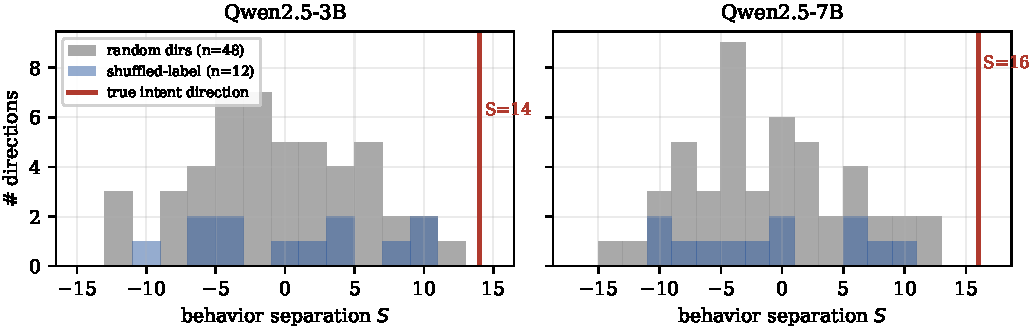
\includegraphics[width=\columnwidth]{specificity.pdf}
\caption{\textbf{The effect requires the learned direction.} Distribution of the behavior separation
$S = \mathrm{feedback}(\text{toward-evaluate}) - \mathrm{feedback}(\text{toward-recognize})$ for $48$ random
directions of matched norm (gray) and $12$ shuffled-label directions (blue), against the true intent direction
(red line). On both models the true direction sits beyond the entire control distribution; no random or
shuffled direction reaches it (permutation $p{=}0.02$).}
\label{fig:specificity}
\end{figure}

\begin{figure}[t]
\centering
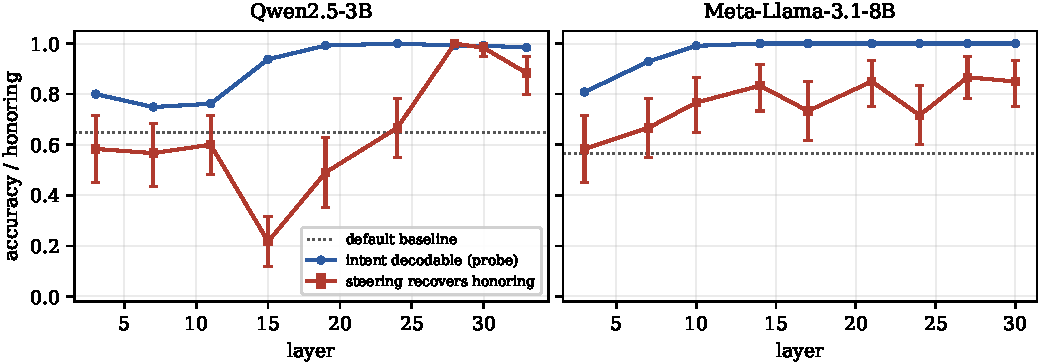
\includegraphics[width=\columnwidth]{localization.pdf}
\caption{\textbf{Represented before routed.} Per layer, how decodable the intent is (blue, probe accuracy) and
how much steering \emph{at that layer} recovers recognize-intent honoring (red, with bootstrap $95\%$ CIs),
against the default baseline (dotted). On both models the probe saturates at layers where steering has not yet
lifted honoring above baseline; recovery arrives only deeper (late and sharp for Qwen-3B, earlier and more
diffuse for Llama-8B). The gap between the blue and red onsets is the discard. $n{=}60$.}
\label{fig:localize}
\end{figure}

\section{Ceiling-model geometry (inconclusive)}
\label{app:geometry}
We asked whether the across-model stratification (Section~\ref{sec:scale}) has a geometric signature: do
the ceiling models, which honor recognize-intent by default, align their intent representation with the readout
more than the discard models do? We pre-registered, before running, the metric $M = |\cos(\text{intent
direction}, \text{readout direction})|$, where the intent direction is the final-layer logistic
recognize-vs-evaluate weight and the readout direction is the fixed acknowledgment-minus-feedback opener
unembedding difference, with the decision rule that the three ceiling models' $M$ must lie clearly above the
three discard models'. \emph{The result does not meet the rule.} Discard models: $M \in \{0.12, 0.06, 0.07\}$;
ceiling models: $\{0.14, 0.30, 0.00\}$. Two of three ceiling models (Mistral $0.30$, Qwen-14B $0.14$) exceed
the discard range, but Phi-3.5 is the lowest of all six ($0.00$), so there is no clean separation; the group
means differ ($0.15$ vs $0.08$) but the pre-registered separation criterion fails. A secondary operationalization
(the direction separating honored from discarded default replies, computable only where both classes occur)
gives $M \le 0.08$ throughout with no pattern. Per our pre-commitment we report the geometry as inconclusive and
make no mechanism claim from it; the across-model claim rests on the behavioral stratification and the
depth localization alone.

\section{Opener-biasing control (full numbers)}
\label{app:opener}
For the deflationary control of Section~\ref{sec:spec}, at each discard model's validated steer layer, matched
activation norm, generating at a $100$-token budget (longer than the $45$-token specificity run so the reply has
a body), we compare four quantities over the same $24$-item subset: $S_{\mathrm{true}}$, the behavior separation
from steering the learned intent direction; $S_{\mathrm{opener}}$, from steering the
acknowledgment-minus-feedback opener-unembedding direction directly; $S_{\mathrm{rest}}$, $S_{\mathrm{true}}$
recomputed with each reply's first sentence removed; and $|\cos|$ between the intent and opener directions at
that layer.

\begin{center}\small
\begin{tabular}{lccccc}
\toprule
model & layer & $S_{\mathrm{true}}$ & $S_{\mathrm{opener}}$ (coherent) & $S_{\mathrm{rest}}$ & $|\cos|$ \\
\midrule
Qwen2.5-7B   & 16 & 14 & $-16$ (only $2/24$ coherent) & 14 & 0.001 \\
Llama-3.1-8B & 19 &  7 & $1$ ($24/24$ coherent, inert) &  4 & 0.034 \\
Qwen2.5-3B   & 30 &  4 & $-1$ (incoherent)            & $-2$ & 0.138 \\
\bottomrule
\end{tabular}
\end{center}

On Qwen-7B the opener direction at matched norm degrades coherence before it honors ($2/24$ coherent), and
$S_{\mathrm{rest}}$ equals the full $S_{\mathrm{true}}$, so intent steering reorients the body, not the opener.
On Llama-8B the longer budget lifts the true separation clear of the random ceiling ($S{=}7$ vs $\max|S|{=}3$)
where the $45$-token run left it tied, the opener direction is inert ($S_{\mathrm{opener}}{=}1$), and
$S_{\mathrm{rest}}{=}4$ shows a modest body effect. On Qwen-3B the true separation \emph{dilutes} at this budget
($S{=}4$, below $\max|S|{=}12$): steered toward acknowledgment the small model acknowledges first but drifts
back into feedback over a long reply (negative-side feedback rises from $3/24$ at $45$ tokens to $17/24$ at
$100$), so the body test is inconclusive on 3B and its refutation rests on the norm-independent
near-orthogonality ($|\cos|{=}0.14$) and the opener direction's incoherence. At the $45$-token budget of
Section~\ref{sec:spec} the 3B separation is strong ($S_{\mathrm{true}}{=}14$), so the dilution is a
generation-length effect, and the intervention on the smallest model is front-loaded. The load-bearing evidence
against opener-biasing is the near-zero cosine on all three models and the body reorientation on Qwen-7B (and,
more modestly, Llama-8B). Script: \texttt{experiments/modal\_opener\_control.py}.

\section{Cross-model direction transport (exploratory)}
\label{app:transport}
The models do not share a hidden size, so a direction cannot transfer verbatim. We fit a linear map from
Qwen-3B activations to Llama-8B activations on a train split of stimuli and transport Qwen's intent direction
into Llama's space. The transported direction lands at cosine $0.85$ to Llama's \emph{own} intent direction,
and steering Llama with it recovers honoring ($0.56 \to 1.00$ on held-out items). We keep this out of the main
text and flag it as exploratory: the map's held-out activation $R^2$ is negative (it aligns the intent
direction, it does not reconstruct activation space), and a random direction of matched norm gives partial
non-specific recovery ($0.69$), so the signal is the direction alignment, not the raw steering number. Read as
suggestive that the intent axis is shared up to a linear map, not as an isomorphism claim.

\section{Request-matched construct control (full numbers)}
\label{app:request}
For the construct-validity control of Section~\ref{sec:repr}, both intent classes carry an explicit directive
so that request-presence is held constant and only the content of the request differs; recognize prefixes
become requests for acknowledgment (``please just celebrate this with me, I really don't want any notes''; ``do
me a favor and just take it in, don't give me feedback''; eight in all), paired with the unchanged evaluate
directives and the same surface-matched suffix. Probe accuracy is leave-one-phrasing-out CV at three depths;
the bag-of-words baseline uses the same phrasing folds.

\begin{center}\small
\begin{tabular}{lcccc}
\toprule
model & probe ($0.5$ / $0.67$ / $0.83$ depth) & peak & bag-of-words \\
\midrule
Qwen2.5-3B   & 0.912 / 0.898 / 0.973 & 0.973 & 0.688 \\
Qwen2.5-7B   & 0.929 / 0.891 / 0.955 & 0.955 & 0.688 \\
Llama-3.1-8B & 0.950 / 0.968 / 0.943 & 0.968 & 0.688 \\
Phi-3.5-mini & 1.000 / 0.984 / 0.953 & 1.000 & 0.688 \\
\bottomrule
\end{tabular}
\end{center}

The probe clears the bag-of-words baseline by roughly $0.25$--$0.30$ on every model with request-presence
matched. The baseline is higher than the surface-matched set's $0.48$ because celebration-requests and
critique-requests use different content words; that residual lexical signal is exactly what the surface-matched
design (Table~\ref{tab:probe}) controls, and the two designs together rule out both confounds. Script:
\texttt{experiments/modal\_request\_matched.py}.

\section{Second intent axis: vent vs solve (full numbers)}
\label{app:axis2}
To test that the represents-discard-recover chain is not specific to the recognize-versus-evaluate contrast, we
replicate it on a different intent: \emph{vent} (``I'm not looking for advice, I just need to be heard'') versus
\emph{solve} (``give me concrete steps to fix this''), behavior scored by whether the reply offers a solution,
surface-matched stimuli built as before on Qwen2.5-3B and Llama-3.1-8B. Intent decodes at probe $1.00$ (Qwen-3B)
and $0.97$ (Llama-8B) at the surface-matched token. At $n{=}60$ with bootstrap CIs, Qwen-3B honors the vent
intent only $0.70$ by default and steering recovers it to $0.98$ (non-overlapping); Llama-8B already honors it
at $0.88$ baseline (ceiling), so steering only nudges it to $0.98$. The representation holds on both; the clean
discard-then-recovery is on the model that discards. This axis is more lexically marked than the first: a
bag-of-words classifier reaches $0.79$ on the full text (versus $0.46$ on recognize-vs-evaluate), so it does
more to show the behavior generalizes to a second intent than to re-establish surface-independent
representation.

\begin{center}\small
\begin{tabular}{lcccc}
\toprule
model & probe & vent honored (default) [95\% CI] & steered [95\% CI] & default vs steered \\
\midrule
Qwen2.5-3B   & 1.00 & 0.70 [0.58, 0.82] & 0.98 [0.95, 1.00] & non-overlapping \\
Llama-3.1-8B & 0.97 & 0.88 [0.80, 0.95] & 0.98 [0.95, 1.00] & ceiling \\
\bottomrule
\end{tabular}
\end{center}

\section{Reproducibility}
\label{app:repro}
\begin{tcolorbox}[graybox, breakable, title={Reproduce}]
\begin{verbatim}
pip install -e .
# core chain (CPU; downloads Qwen2.5-3B-Instruct)
python experiments/probe_intent.py        # represents (leave-phrasing-out)
python experiments/same_model_discard.py  # discards (same model)
python experiments/steer_probe_sweep.py   # find the causal layer
python experiments/steer_dose.py          # dose-response confirmation
pytest                                     # pipeline + no-leak guards
# extended experiments (GPU, via Modal)
modal run experiments/modal_sweep.py      # generality ladder (6 models)
modal run experiments/modal_scale.py      # discard/recover at n=60 with bootstrap CIs
modal run experiments/modal_specificity2.py  # norm-matched + shuffled controls
modal run experiments/modal_localize2.py  # depth localization, n=60 + CIs, two models
modal run experiments/modal_natural.py    # naturalistic transfer
\end{verbatim}
\end{tcolorbox}
The core probe is CPU-only and downloads Qwen2.5-3B-Instruct; the extended experiments run on a single
A100 through Modal (\url{https://modal.com}), and the behavioral elicitation uses API keys. Code, stimuli, and
all experiment scripts are available at \url{https://github.com/collapseindex/recipient-probe}.

\paragraph{Software.} Experiments use PyTorch \citep{paszke2019pytorch}, HuggingFace Transformers
\citep{wolf2020transformers}, scikit-learn \citep{pedregosa2011sklearn} for the probes and steering fits, and
sentence-transformers \citep{reimers2019sbert} for the independent embedding measure (Section~\ref{sec:discard}).

\end{document}